
%% bare_conf.tex
%% V1.3
%% 2007/01/11
%% by Michael Shell
%% See:
%% http://www.michaelshell.org/
%% for current contact information.
%%
%% This is a skeleton file demonstrating the use of IEEEtran.cls
%% (requires IEEEtran.cls version 1.7 or later) with an IEEE conference paper.
%%
%% Support sites:
%% http://www.michaelshell.org/tex/ieeetran/
%% http://www.ctan.org/tex-archive/macros/latex/contrib/IEEEtran/
%% and
%% http://www.ieee.org/

%%*************************************************************************
%% Legal Notice:
%% This code is offered as-is without any warranty either expressed or
%% implied; without even the implied warranty of MERCHANTABILITY or
%% FITNESS FOR A PARTICULAR PURPOSE! 
%% User assumes all risk.
%% In no event shall IEEE or any contributor to this code be liable for
%% any damages or losses, including, but not limited to, incidental,
%% consequential, or any other damages, resulting from the use or misuse
%% of any information contained here.
%%
%% All comments are the opinions of their respective authors and are not
%% necessarily endorsed by the IEEE.
%%
%% This work is distributed under the LaTeX Project Public License (LPPL)
%% ( http://www.latex-project.org/ ) version 1.3, and may be freely used,
%% distributed and modified. A copy of the LPPL, version 1.3, is included
%% in the base LaTeX documentation of all distributions of LaTeX released
%% 2003/12/01 or later.
%% Retain all contribution notices and credits.
%% ** Modified files should be clearly indicated as such, including  **
%% ** renaming them and changing author support contact information. **
%%
%% File list of work: IEEEtran.cls, IEEEtran_HOWTO.pdf, bare_adv.tex,
%%                    bare_conf.tex, bare_jrnl.tex, bare_jrnl_compsoc.tex
%%*************************************************************************

% *** Authors should verify (and, if needed, correct) their LaTeX system  ***
% *** with the testflow diagnostic prior to trusting their LaTeX platform ***
% *** with production work. IEEE's font choices can trigger bugs that do  ***
% *** not appear when using other class files.                            ***
% The testflow support page is at:
% http://www.michaelshell.org/tex/testflow/



% Note that the a4paper option is mainly intended so that authors in
% countries using A4 can easily print to A4 and see how their papers will
% look in print - the typesetting of the document will not typically be
% affected with changes in paper size (but the bottom and side margins will).
% Use the testflow package mentioned above to verify correct handling of
% both paper sizes by the user's LaTeX system.
%
% Also note that the "draftcls" or "draftclsnofoot", not "draft", option
% should be used if it is desired that the figures are to be displayed in
% draft mode.
%
\documentclass[conference,a4paper]{IEEEtran}
% Add the compsoc option for Computer Society conferences.
%
% If IEEEtran.cls has not been installed into the LaTeX system files,
% manually specify the path to it like:
% \documentclass[conference]{../sty/IEEEtran}





% Some very useful LaTeX packages include:
% (uncomment the ones you want to load)


% *** MISC UTILITY PACKAGES ***
%
%\usepackage{ifpdf}
% Heiko Oberdiek's ifpdf.sty is very useful if you need conditional
% compilation based on whether the output is pdf or dvi.
% usage:
% \ifpdf
%   % pdf code
% \else
%   % dvi code
% \fi
% The latest version of ifpdf.sty can be obtained from:
% http://www.ctan.org/tex-archive/macros/latex/contrib/oberdiek/
% Also, note that IEEEtran.cls V1.7 and later provides a builtin
% \ifCLASSINFOpdf conditional that works the same way.
% When switching from latex to pdflatex and vice-versa, the compiler may
% have to be run twice to clear warning/error messages.






% *** CITATION PACKAGES ***
%
\usepackage{cite}
% cite.sty was written by Donald Arseneau
% V1.6 and later of IEEEtran pre-defines the format of the cite.sty package
% \cite{} output to follow that of IEEE. Loading the cite package will
% result in citation numbers being automatically sorted and properly
% "compressed/ranged". e.g., [1], [9], [2], [7], [5], [6] without using
% cite.sty will become [1], [2], [5]--[7], [9] using cite.sty. cite.sty's
% \cite will automatically add leading space, if needed. Use cite.sty's
% noadjust option (cite.sty V3.8 and later) if you want to turn this off.
% cite.sty is already installed on most LaTeX systems. Be sure and use
% version 4.0 (2003-05-27) and later if using hyperref.sty. cite.sty does
% not currently provide for hyperlinked citations.
% The latest version can be obtained at:
% http://www.ctan.org/tex-archive/macros/latex/contrib/cite/
% The documentation is contained in the cite.sty file itself.






% *** GRAPHICS RELATED PACKAGES ***
%
\ifCLASSINFOpdf
   \usepackage[pdftex]{graphicx}
  % declare the path(s) where your graphic files are
   \graphicspath{{figures/}}%{../jpeg/}}
  % and their extensions so you won't have to specify these with
  % every instance of \includegraphics
   \DeclareGraphicsExtensions{.pdf,.jpeg,.png}
\else
  % or other class option (dvipsone, dvipdf, if not using dvips). graphicx
  % will default to the driver specified in the system graphics.cfg if no
  % driver is specified.
  % \usepackage[dvips]{graphicx}
  % declare the path(s) where your graphic files are
  % \graphicspath{{../eps/}}
  % and their extensions so you won't have to specify these with
  % every instance of \includegraphics
  % \DeclareGraphicsExtensions{.eps}
\fi
% graphicx was written by David Carlisle and Sebastian Rahtz. It is
% required if you want graphics, photos, etc. graphicx.sty is already
% installed on most LaTeX systems. The latest version and documentation can
% be obtained at: 
% http://www.ctan.org/tex-archive/macros/latex/required/graphics/
% Another good source of documentation is "Using Imported Graphics in
% LaTeX2e" by Keith Reckdahl which can be found as epslatex.ps or
% epslatex.pdf at: http://www.ctan.org/tex-archive/info/
%
% latex, and pdflatex in dvi mode, support graphics in encapsulated
% postscript (.eps) format. pdflatex in pdf mode supports graphics
% in .pdf, .jpeg, .png and .mps (metapost) formats. Users should ensure
% that all non-photo figures use a vector format (.eps, .pdf, .mps) and
% not a bitmapped formats (.jpeg, .png). IEEE frowns on bitmapped formats
% which can result in "jaggedy"/blurry rendering of lines and letters as
% well as large increases in file sizes.
%
% You can find documentation about the pdfTeX application at:
% http://www.tug.org/applications/pdftex





% *** MATH PACKAGES ***
%
\usepackage[cmex10]{amsmath}
% A popular package from the American Mathematical Society that provides
% many useful and powerful commands for dealing with mathematics. If using
% it, be sure to load this package with the cmex10 option to ensure that
% only type 1 fonts will utilized at all point sizes. Without this option,
% it is possible that some math symbols, particularly those within
% footnotes, will be rendered in bitmap form which will result in a
% document that can not be IEEE Xplore compliant!
%
% Also, note that the amsmath package sets \interdisplaylinepenalty to 10000
% thus preventing page breaks from occurring within multiline equations. Use:
%\interdisplaylinepenalty=2500
% after loading amsmath to restore such page breaks as IEEEtran.cls normally
% does. amsmath.sty is already installed on most LaTeX systems. The latest
% version and documentation can be obtained at:
% http://www.ctan.org/tex-archive/macros/latex/required/amslatex/math/


\usepackage{siunitx}



% *** SPECIALIZED LIST PACKAGES ***
%
\usepackage{algorithm}
\usepackage{algorithmic}
% algorithmic.sty was written by Peter Williams and Rogerio Brito.
% This package provides an algorithmic environment fo describing algorithms.
% You can use the algorithmic environment in-text or within a figure
% environment to provide for a floating algorithm. Do NOT use the algorithm
% floating environment provided by algorithm.sty (by the same authors) or
% algorithm2e.sty (by Christophe Fiorio) as IEEE does not use dedicated
% algorithm float types and packages that provide these will not provide
% correct IEEE style captions. The latest version and documentation of
% algorithmic.sty can be obtained at:
% http://www.ctan.org/tex-archive/macros/latex/contrib/algorithms/
% There is also a support site at:
% http://algorithms.berlios.de/index.html
% Also of interest may be the (relatively newer and more customizable)
% algorithmicx.sty package by Szasz Janos:
% http://www.ctan.org/tex-archive/macros/latex/contrib/algorithmicx/




% *** ALIGNMENT PACKAGES ***
%
%\usepackage{array}
% Frank Mittelbach's and David Carlisle's array.sty patches and improves
% the standard LaTeX2e array and tabular environments to provide better
% appearance and additional user controls. As the default LaTeX2e table
% generation code is lacking to the point of almost being broken with
% respect to the quality of the end results, all users are strongly
% advised to use an enhanced (at the very least that provided by array.sty)
% set of table tools. array.sty is already installed on most systems. The
% latest version and documentation can be obtained at:
% http://www.ctan.org/tex-archive/macros/latex/required/tools/


%\usepackage{mdwmath}
%\usepackage{mdwtab}
% Also highly recommended is Mark Wooding's extremely powerful MDW tools,
% especially mdwmath.sty and mdwtab.sty which are used to format equations
% and tables, respectively. The MDWtools set is already installed on most
% LaTeX systems. The lastest version and documentation is available at:
% http://www.ctan.org/tex-archive/macros/latex/contrib/mdwtools/


% IEEEtran contains the IEEEeqnarray family of commands that can be used to
% generate multiline equations as well as matrices, tables, etc., of high
% quality.


%\usepackage{eqparbox}
% Also of notable interest is Scott Pakin's eqparbox package for creating
% (automatically sized) equal width boxes - aka "natural width parboxes".
% Available at:
% http://www.ctan.org/tex-archive/macros/latex/contrib/eqparbox/





% *** SUBFIGURE PACKAGES ***
%\usepackage[tight,footnotesize]{subfigure}
% subfigure.sty was written by Steven Douglas Cochran. This package makes it
% easy to put subfigures in your figures. e.g., "Figure 1a and 1b". For IEEE
% work, it is a good idea to load it with the tight package option to reduce
% the amount of white space around the subfigures. subfigure.sty is already
% installed on most LaTeX systems. The latest version and documentation can
% be obtained at:
% http://www.ctan.org/tex-archive/obsolete/macros/latex/contrib/subfigure/
% subfigure.sty has been superceeded by subfig.sty.


%\usepackage{graphicx}
%\graphicspath{{figures/}}
%\usepackage[caption=false]{caption}
%\usepackage[font=footnotesize]{subfig}
% subfig.sty, also written by Steven Douglas Cochran, is the modern
% replacement for subfigure.sty. However, subfig.sty requires and
% automatically loads Axel Sommerfeldt's caption.sty which will override
% IEEEtran.cls handling of captions and this will result in nonIEEE style
% figure/table captions. To prevent this problem, be sure and preload
% caption.sty with its "caption=false" package option. This is will preserve
% IEEEtran.cls handing of captions. Version 1.3 (2005/06/28) and later 
% (recommended due to many improvements over 1.2) of subfig.sty supports
% the caption=false option directly:
%\usepackage[caption=false,font=footnotesize]{subfig}
%
% The latest version and documentation can be obtained at:
% http://www.ctan.org/tex-archive/macros/latex/contrib/subfig/
% The latest version and documentation of caption.sty can be obtained at:
% http://www.ctan.org/tex-archive/macros/latex/contrib/caption/




% *** FLOAT PACKAGES ***
%
%\usepackage{fixltx2e}
% fixltx2e, the successor to the earlier fix2col.sty, was written by
% Frank Mittelbach and David Carlisle. This package corrects a few problems
% in the LaTeX2e kernel, the most notable of which is that in current
% LaTeX2e releases, the ordering of single and double column floats is not
% guaranteed to be preserved. Thus, an unpatched LaTeX2e can allow a
% single column figure to be placed prior to an earlier double column
% figure. The latest version and documentation can be found at:
% http://www.ctan.org/tex-archive/macros/latex/base/



%\usepackage{stfloats}
% stfloats.sty was written by Sigitas Tolusis. This package gives LaTeX2e
% the ability to do double column floats at the bottom of the page as well
% as the top. (e.g., "\begin{figure*}[!b]" is not normally possible in
% LaTeX2e). It also provides a command:
%\fnbelowfloat
% to enable the placement of footnotes below bottom floats (the standard
% LaTeX2e kernel puts them above bottom floats). This is an invasive package
% which rewrites many portions of the LaTeX2e float routines. It may not work
% with other packages that modify the LaTeX2e float routines. The latest
% version and documentation can be obtained at:
% http://www.ctan.org/tex-archive/macros/latex/contrib/sttools/
% Documentation is contained in the stfloats.sty comments as well as in the
% presfull.pdf file. Do not use the stfloats baselinefloat ability as IEEE
% does not allow \baselineskip to stretch. Authors submitting work to the
% IEEE should note that IEEE rarely uses double column equations and
% that authors should try to avoid such use. Do not be tempted to use the
% cuted.sty or midfloat.sty packages (also by Sigitas Tolusis) as IEEE does
% not format its papers in such ways.

% *** PDF, URL AND HYPERLINK PACKAGES ***
%
\usepackage[obeyspaces]{url}
\usepackage{hyperref}% http://ctan.org/pkg/hyperref
% url.sty was written by Donald Arseneau. It provides better support for
% handling and breaking URLs. url.sty is already installed on most LaTeX
% systems. The latest version can be obtained at:
% http://www.ctan.org/tex-archive/macros/latex/contrib/misc/
% Read the url.sty source comments for usage information. Basically,
% \url{my_url_here}.

% Advanced table environment
\usepackage{booktabs}

\usepackage{lipsum}



% *** Do not adjust lengths that control margins, column widths, etc. ***
% *** Do not use packages that alter fonts (such as pslatex).         ***
% There should be no need to do such things with IEEEtran.cls V1.6 and later.
% (Unless specifically asked to do so by the journal or conference you plan
% to submit to, of course. )


% correct bad hyphenation here
\hyphenation{op-tical net-works semi-conduc-tor ar-ti-ficial in-telli-gence conscious-thought}


\begin{document}
%
% paper title
% can use linebreaks \\ within to get better formatting as desired
%\title{Survey paper: \\Artificial Intelligence for optimisation of HVAC-systems}
\title{The Development and Comparison of Algorithms towards an Autonomous F1/10-Car}


% author names and affiliations
% use a multiple column layout for up to three different
% affiliations

%\author{\IEEEauthorblockN{Jens de Hoog}
%\IEEEauthorblockA{Department of Applied Engineering \\Electronics-ICT\\
%University of Antwerp\\
%Antwerp, Belgium\\
%jens.dehoog@student.uantwerpen.be}
%\and
%\IEEEauthorblockN{Maggy Goossens}
%\IEEEauthorblockA{Department of Applied Engineering \\Electronics-ICT\\
%University of Antwerp\\
%Antwerp, Belgium\\
%maggy.goossens@uantwerpen.be}
%\and
%\IEEEauthorblockN{Peter Hellinckx}
%\IEEEauthorblockA{Department of Applied Engineering \\Electronics-ICT\\
%University of Antwerp\\
%Antwerp, Belgium\\
%peter.hellinckx@uantwerpen.be}
%}

\author{
\IEEEauthorblockN{Jens de Hoog\IEEEauthorrefmark{1},
		Thomas Huybrechts\IEEEauthorrefmark{1}\IEEEauthorrefmark{4},
		Ben Bellekens\IEEEauthorrefmark{1}\IEEEauthorrefmark{4},
		Peter Hellinckx\IEEEauthorrefmark{1}\IEEEauthorrefmark{4}\\
	jens.dehoog@student.uantwerpen.be, thomas.huybrechts@uantwerpen.be,\\ ben.bellekens@uantwerpen.be, peter.hellinckx@uantwerpen.be}
	\\\IEEEauthorblockA{
	    \IEEEauthorrefmark{1}Faculty of Applied Engineering, Electronics-ICT, University of Antwerp, Belgium
	}
	\IEEEauthorblockA{
	    \IEEEauthorrefmark{4}University of Antwerp - imec, IDLab, Faculty of Applied Engineering, Belgium
	}
}

% make the title area
\maketitle

\begin{abstract}
%\boldmath
\lipsum[1]

\end{abstract}
% IEEEtran.cls defaults to using nonbold math in the Abstract.
% This preserves the distinction between vectors and scalars. However,
% if the conference you are submitting to favors bold math in the abstract,
% then you can use LaTeX's standard command \boldmath at the very start
% of the abstract to achieve this. Many IEEE journals/conferences frown on
% math in the abstract anyway.

% no keywords

% For peer review papers, you can put extra information on the cover
% page as needed:
% \ifCLASSOPTIONpeerreview
% \begin{center} \bfseries EDICS Category: 3-BBND \end{center}
% \fi
%
% For peerreview papers, this IEEEtran command inserts a page break and
% creates the second title. It will be ignored for other modes.
\IEEEpeerreviewmaketitle



\section{Introduction}
%Despite the fact that artificial intelligence (AI) is not a new concept, it has become increasingly popular these days. Its first goal was to let machines replicate the intelligence of a human being, but that goal appeared to be more difficult than researches thought it would be. Slow progress was made for the next years, but technology has become more powerful and the interest in AI increased again, especially in marketable aspects\cite{Brooks1991}. At present, AI is quite ubiquitous and is implemented in many topics, such as self-driving cars. \\

%*Moet nog uitgebreid worden*

%\lipsum[2-4]

%\section{**Testopstelling¨**}
%\subsection{F1/10-car}
%Ik vertel over de wagen in het algemeen en welke sensoren eropzitten. Dit gebeurt heel kort.
%Ook vertel ik over de globale structuur van ROS en welke belangrijke nodes er gebruikt worden.
%
%\subsection{Prerequisites}
%In dit deel vertel ik over het traag rijden en het rijden tegen constante snelheid.
%\begin{itemize}
%\item Slow accurate driving: er wordt een beetje aandacht besteedt aan de twee approaches en waarom ze wel/niet werkten
%\item Ik vertel kort waarom het rijden op softwareniveau (met IMU) niet werkten en hoe het met de RPM-sensor is opgelost.
%\end{itemize}

The original intent of the F1/10-car was to develop an autonomous race car which would compete against other cars, each with other algorithms. The University of Pennsylvania \cite{f1tenth} published multiple tutorials, lessons and exercises in order to set up an F1/10-car from the very beginning. Additionally, the university proposes several algorithms which can be used to drive on a race track. Though, these algorithms are optimised for racing on fixed tracks at high speeds. 

\section{Algorithms}
\subsection{Global outline}
 
In order to navigate in a particular environment, multiple methods of navigation exist. In this paper, three approaches are discussed. A small literature study is made for each approach, along with an explanation of the algorithm itself and a discussion of the obtained results.

In the first method, the car drives on a fixed trajectory which was calculated in advance. The second approach deals with waypoints. Thus, the car has to drive along these points in order to reach the destination. It is worth noting that no path is calculated between the waypoints. Otherwise, the first method is approached. Only a destination is given in the third and last process such that the car has to find the destination itself. 

\subsection{Fixed path}
%\begin{description}
%\item[Literature] \hfill \\ In dit deel leg ik verschillende globale algoritmes naast elkaar. Ook vertel ik dat de Navigation Stack aanwezig is in ROS en dat deze daa

%\item[Navigation Stack] \hfill \\ Hierin vertel ik dat er een implementatie bestaat in het ROS-framework, hoe deze is opgebouwd (subnodes, lokale / globale planner, AMCL, \ldots), wat er is foutgelopen bij het opzetten van de Stack en wat de oplossingen daarvoor waren. Ook vertelt dit deel over het feit dat de Stack in principe gemaakt is voor een differenti\"{e}le of holonomische sturing. Oplossingen worden daarvoor aangereikt, samen met de uitleg waarom die oplossingen goed/slecht waren.
%Het ‘foutgelopen+oplossingen’-deel is beknopt. De oplossingen worden aangereikt in een korte maar duidelijke manier. 

%\item[Resultaten] \hfill \\ Dit deel vertelt over het verloop van het navigeren d.m.v. de Stack. Er komen foto’s aan bod van het uitgestippelde pad, de auto die tegen de muur zit, \ldots

%\end{description}
In the state-of-the-art, considerable research has been done in planning a particular route and navigating on that route. Henson et al. \cite{Henson2008} propose an algorithm which processes waypoint instructions by calculating a route between each point. This algorithm is optimised for cars with an Ackermann-steering mechanism. Thus, if the waypoint is reached but without the requested orientation, the car starts to manoeuvre until the positioning is correct. 

Theodosis \cite{Theodosis2014} suggests multiple methods, all of which use waypoints. These checkpoints are connected with racing lines such that a car-like robot can easily navigate without impossible pivot points. 

In the ROS-framework, a complete navigator package is available, which is also known as the \emph{Navigation Stack}. This module calculates a path and velocity commands based on given information, such as odometry and data from rangefinders. A major drawback of this navigator is the fact that it is created for robots with holonomic and differential steering mechanisms. Though, it is usable for car-like robots as there exist implementations for Ackermann-steering mechanisms.

For this research, the navigation stack has been implemented. It is easy to set up on the F1/10-car as the software on the car is already running a ROS-environment.
The module is realised using multiple nodes and packages. One of these nodes is the \emph{move\textunderscore base}-node, which has a major role in the system. This node provides the linkage between the global and local planning algorithms that are used to calculate a path from the start location to the destination. Other nodes outside the package provide the inputs and outputs of the \emph{move\textunderscore base}-node. The needed inputs are the odometry data, transformations, localisation information, the map on which the navigation would take place and the data from a certain rangefinder. In our setup, a LiDAR-sensor (Light Detection and Ranging) serves as rangefinder. The commands by which the car would drive, are the generated outputs of the central navigation node. Figure \ref{fig:navstack_global} shows an overall overview of the different nodes in the navigation stack \cite{Marder-Eppstein2016}. 

Inside the \textit{move\textunderscore base}-node, multiple calculations take place in order to navigate. First, a plugin called \emph{global\textunderscore costmap} produces a costmap, which is used to plan the route from start to destination. This is done by the plugin \emph{global\textunderscore planner}. The default implementation of this planner is \emph{navfn}. In our implementation, we opted for the more advanced planner \emph{global\textunderscore planner} because of the ability to customise multiple parameters. Second, the central node produces a local costmap which is used by the local planner. By using this particular costmap and planner, the navigation stack is able to plan a route around an unexpected obstacle that is not present on the map. The default local planner is \emph{base\textunderscore local\textunderscore planner}. Though, an other implementation is available for car-like robots. This planner is known as \emph{teb\textunderscore local\textunderscore planner}\cite{Rosmann2016}.  As a safety feature, the \emph{move\textunderscore base}-node includes a recovery plugin which plans a secondary route when the car is stuck and thus unable to follow the planned route.
Figure \ref{fig:navstack_global} shows an abstract overview of the navigation stack with its nodes and plugins \cite{Marder-Eppstein2016_2, Zheng2016}.
\begin{figure}[!t]
    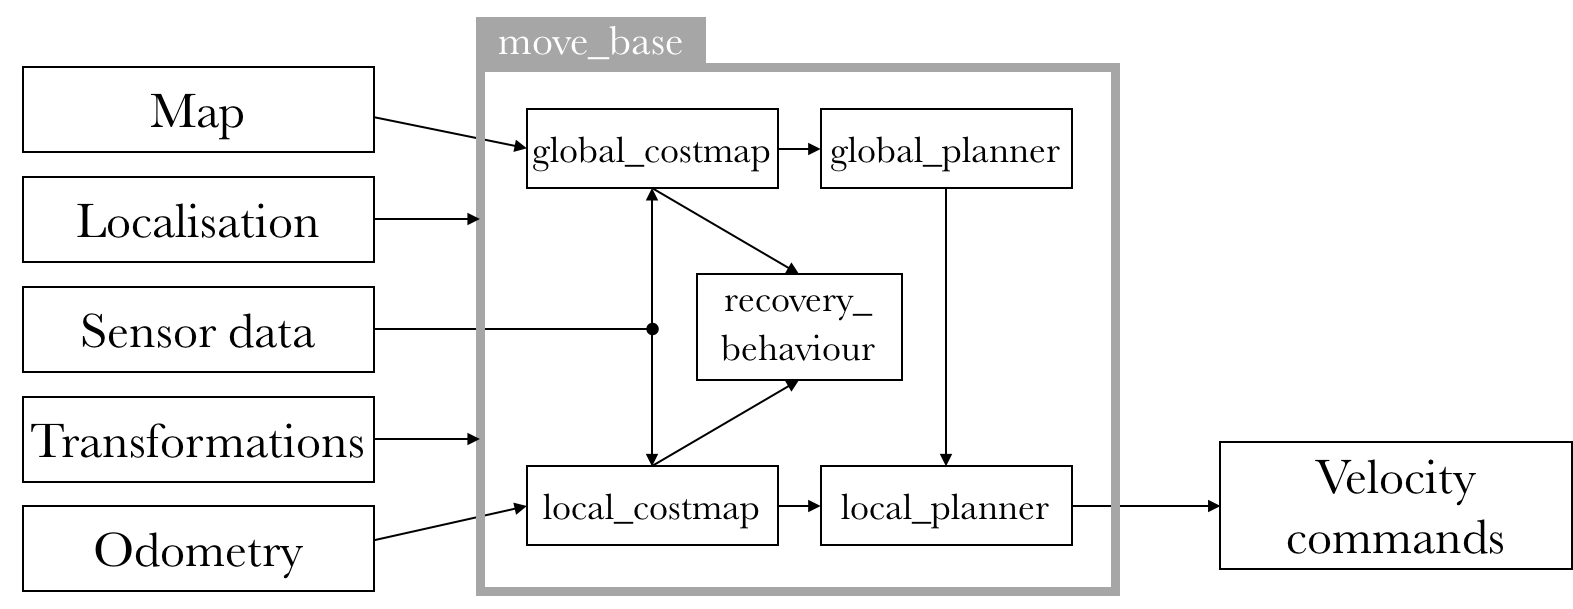
\includegraphics[width=\columnwidth]{navstack3}
    \centering
    \caption{Overview of the navigation stack with its input and output nodes, along with the plugins inside the \emph{move\textunderscore base}-node \cite{Marder-Eppstein2016}.}
    \label{fig:navstack_global}
\end{figure}

Before the car is able to drive using the navigation stack, one has to make sure a map of the environment is present. The map used in this research is built by using \emph{hector\textunderscore mapping}. This package is an implementation of the SLAM-methodology (Simultaneous Localisation And Mapping), which only uses data from the LiDAR-sensor. Therefore, this is the most suitable implementation for our F1/10-car due to the lack of odometry data. An elaborated discussion on \emph{hector\textunderscore mapping} can be found in \cite{Kohlbrecher2011} and \cite{Kohlbrecher2012}. 

In order to use the \emph{move\textunderscore base}-node properly, certain precautions have to be made. First, the transformation tree has to be correct such that the laser data can be transformed to the center of the robot. To build such a tree, two \emph{tf}-nodes are created. The first node transforms the LiDAR-data to a link that connects all types of sensors. The second node transforms the linking point to the center of the frame. Since only one sensor is present, we locate the linking point to the center of the frame; thus, the second transformation is one-to-one. Though, this second transform is needed as the navigation stack needs the \emph{base\textunderscore frame}-transformation \cite{Kohlbrecher2012_tf} \cite{Woodall2015}.

Second, the navigation stack needs a source of odometry data. Since the car does not feature a suitable source, we have to generate such data from the LiDAR-sensor. \emph{Hector\textunderscore mapping} has the ability to provide odometry data which is derived from the laser scan. In order to use this data in the navigation stack, a particular node is needed which translates the odometry information to transformation data. The implementation of this node is available on the \emph{f1tenth}-repository of Nischal K.N. \cite{K.N.2016}.

Third, the robot must be able to guess its location on the given map. This is implemented by the \emph{AMCL}-node (\emph{Adaptive Monte Carlo Localisation}). In order to generate a suitable pose guess, the node also needs odometry data, along with the map, transformations and LiDAR-information \cite{Gerkey2016} \cite{Thrun1999}. The pose guess is relative to the given map; thus, this node provides the transformation between the odometry and the map.\\
Final, the translation from the velocity commands of the navigator to instructions for the motor controller needs to be made.
Figure \ref{fig:navstack_tf} shows the transformations created by the aforementioned nodes. 

\begin{figure}[!t]
    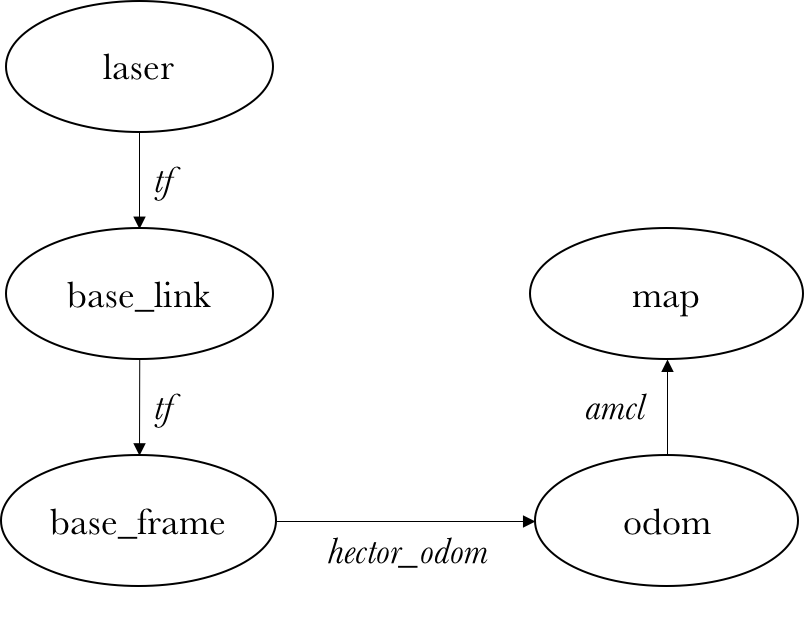
\includegraphics[width=\columnwidth]{navstack_tf}
    \centering
    \caption{Created transformation frames for the navigation stack. The \emph{tf}-links between \emph{laser}, \emph{base\textunderscore link} and \emph{base\textunderscore frame} are static transforms. Next, the \emph{hector\textunderscore odom}-link is created by a node which translates the odometry of \emph{hector\textunderscore mapping}. The \emph{amcl}-transform is created by the localisation provider.}
    \label{fig:navstack_tf}
\end{figure}

\begin{figure}[!t]
	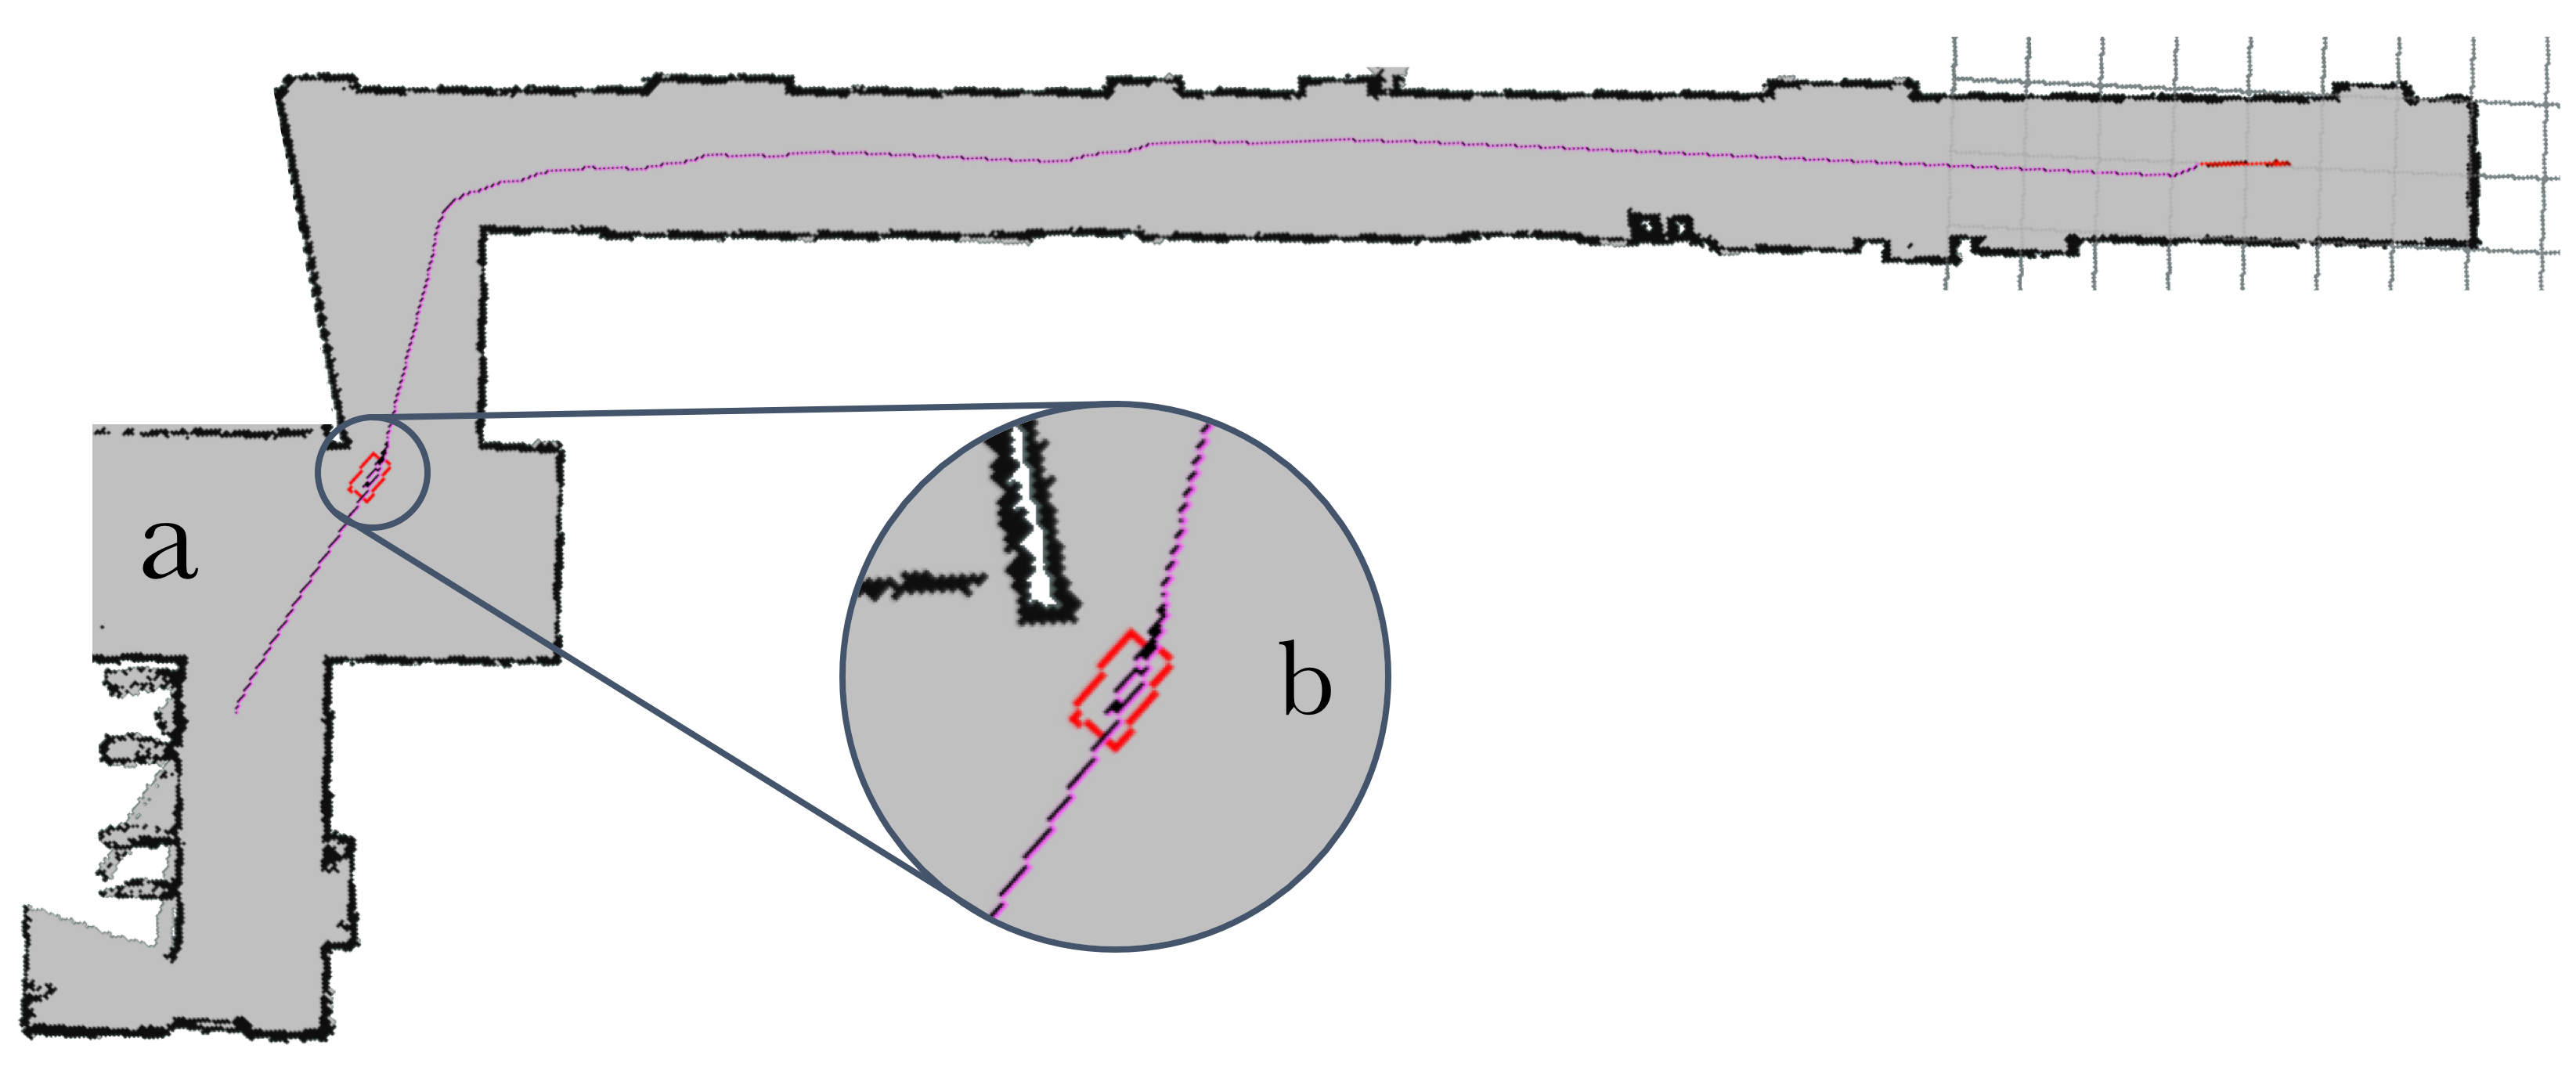
\includegraphics[width=\columnwidth]{navstack_result_1}
	\centering
	\caption{a) shows the route which is planned by the navigation stack. The map is built with \emph{hector\textunderscore mapping}\cite{Kohlbrecher2012}. b) illustrates a close-up of the car moving on the route. }
	\label{fig:navstack_result}
\end{figure}

As a result, the planned route is shown in figure \ref{fig:navstack_result}, along with a close-up of the car navigating on that path. 

A major drawback of the navigation stack is its lack of optimisation for car-like robots. Instead, it is especially created for robots with holonomic or differential steering mechanisms. Therefore, the car is sometimes unable to follow the calculated path. Because of this problem, we implemented \emph{teb\textunderscore local\textunderscore planner} such that the route would be more optimised for Ackermann-steering. It appeared that this planner needed a a lot of computing power. The onboard NVIDIA Jetson TK1 was unable to finish the calculations before the requested deadlines. Even a virtual machine with high specifications could not finish the process. Therefore, the default local planner is used for further usage. Although using this planner could result in pivot points and sharp curves, the car is perfectly able to navigate on the trajectory if the curves are almost straight and without turning points.
Another drawback is the low driving speed at which the car has to drive in order to update its position. By increasing speed, a certain latency exists between the actual position and the calculated one. As a result, the navigation stack is too slow with processing a new local path and crashes could occur.
%Using this planner results in pivot points and curves; thus the car is unable to follow those parts of the path. 

\subsection{Waypoints}
%\begin{description}
%\item[Literature] \hfill \\ In dit deel komen verschillende algoritmes naar boven die in de literatuur te vinden zijn. Ook wordt er gezegd waarom deze algoritmes niet goed genoeg zijn voor mijn doel en dat ik daarom zelf een algoritme heb ontwikkeld.
%
%\item[Concept] \hfill \\ Deze paragraaf legt het algoritme uit, samen met alle edge cases (wat als een muur wegvalt, wat als ik een kruispunt tegenkom, \ldots).
%
%\item[Resultaten] \hfill \\ Dit deel beschrijft de resultaten. Hierin komt ook aan bod dat het algoritme in het algmeen goed werkt, maar dat de LiDAR-sensor gevoelig is aan de soort reflectie (zwarte voorwerpen hebben minder reflectie) en dat er daardoor veel afstelwerk vereist was. Dit komt ook aan bod in “further research”.
%
%\end{description}

In the current state-of-the-art, many navigation algorithms process waypoints in order to reach the destination. E.g., the aforementioned algorithms \cite{Henson2008}\cite{Theodosis2014} use waypoints to describe the route, but the paths between those points are still calculated; thus these algorithms are suitable for the fixed path approach mentioned in the previous section. Due to the lack of research for this problem, no acceptable solutions are available yet. Therefore, this paper suggests a new methodology to tackle this problem.

%Before we shed light on the actual algorithm, a few notes have to be made. First, 
%The algorithm is similar to \emph{turn-by-turn}-navigation used in GPS-systems. 
In the algorithm, a waypoint is similar to an instruction of  \emph{turn-by-turn}-based navigation. A waypoint consists of two datafields: \emph{direction} and \emph{count}.
The \emph{direction}-field has three possible options: \emph{straigt}, \emph{left} and \emph{right}. The \emph{count}-variable describes which turn should be taken. Figure \ref{fig:waypoints_turns} shows two examples. In the first case, the waypoint is described as $(\text{\emph{right}},\,2)$. I.e., the car should take the second exit on the right. The instruction of the second example is described as $(\text{\emph{left}},\,3)$. 

\begin{figure}[!t]
	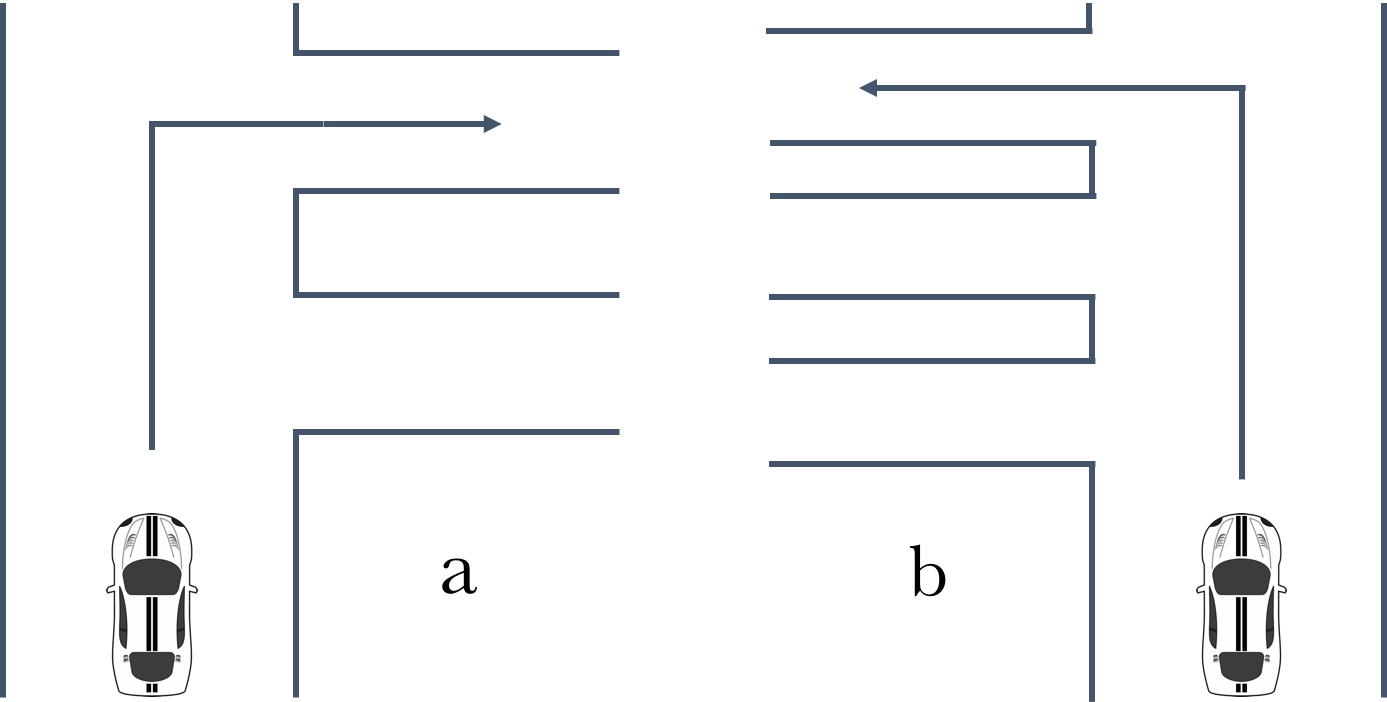
\includegraphics[width=\columnwidth]{waypoints_turns}
	\centering
	\caption{a) illustrates a waypoint which is described as $(\text{\emph{right}},\,2)$. b) shows the instruction $(\text{\emph{left}},\,3)$. }
	\label{fig:waypoints_turns}
\end{figure}

The actual implementation of the algorithm is done by B. Smits and S. Maes for their bachelor's thesis, but first, a few prerequisites have to be made. We have to make sure the car drives in the middle of the road in order to drive in a hallway. Smits and Maes implemented multiple ROS-nodes which adjust the wheel position of the car by given LiDAR-data, thus regulating the distance with respect to the wall while driving. 

With this ROS-nodes, the implementation of the algorithm takes place. When the car is driving and it detects a corner on one of its sides, the software checks if this is the corner that is specified by the waypoint instruction. If false, the car continues driving while focusing on the opposite wall, such that the car stays in the middle of the road. If the result is true, the car will take the turn by adjusting the wheel position until the car is parallel with the wall of the corner. If the software detects corners on both of its sides, but neither of them is specified by the waypoint, the steering position is set to neutral. Therefore, the car drives straight until a wall on either side is detected. Thus, the aforementioned ROS-nodes can be resumed.

%\begin{algorithm}
%	\caption{Waypoint Navigation}
%	\label{alg:waypoint_navigation}
%\begin{algorithmic}
%    \STATE $Waypoint \leftarrow (direction, count)$
%	\STATE Fill list $Waypoint[]$
%\end{algorithmic}
%\begin{algorithmic}[1]
%	\REQUIRE $Waypoint[]$
%	\WHILE{list $Waypoint[]$ is not empty}
%	\STATE $point \leftarrow \text{Read element from} Waypoint[]$
%	\STATE 
%	\ENDWHILE
%\end{algorithmic}
%\end{algorithm}
%As mentioned in the paragraph \emph{Literature} of previous section, multiple navigation algorithms using waypoints are already developed. Though, paths are still calculated between those waypoints. Thus, the previous section is approached by these algorithms. 

\paragraph{Concept}
%\begin{algorithmic}[1]
%	\WHILE{list of waypoints is not $0$}
%	\STATE carry out some processing
%	\ENDWHILE
%\end{algorithmic}

\subsection{Optimisation Algorithm}
\begin{description}
\item[Literature] \hfill \\ Ik leg verschillende algoritmes naast elkaar en maak een kleine vergelijkende studie. Ik leg ook uit waarom ik een bepaald algoritme heb gekozen.

\item[Concept] \hfill \\ Het gekozen algoritme wordt in meer in detail besproken.

\item[Resultaten] \hfill \\ De resultaten van dit algoritme wordt besproken.

\end{description}

\section{Comparative study}
De hierboven voorgelegde approaches worden met elkaar vergeleken en er worden verschillende toepassingen opgesomd waarin elk algoritme faalt of uitblinkt.

\section{Test setup}
\subsection{F1/10-car}
Ik vertel over de wagen in het algemeen en welke sensoren eropzitten. Dit gebeurt heel kort.
Ook vertel ik over de globale structuur van ROS en welke belangrijke nodes er gebruikt worden.

\subsection{Prerequisites}
In dit deel vertel ik over het traag rijden en het rijden tegen constante snelheid.
\begin{itemize}
\item Slow accurate driving: er wordt een beetje aandacht besteedt aan de twee approaches en waarom ze wel/niet werkten
\item Ik vertel kort waarom het rijden op softwareniveau (met IMU) niet werkten en hoe het met de RPM-sensor is opgelost.
\end{itemize}

\section{Conclusion}
De conclusie wordt gemaakt.

\section{Further Research}
In dit deel wordt kort besproken wat er allemaal nog gedaan kan worden van research. Er kan bijvoorbeeld gekeken naar worden optimalisaties voor de Navigation Stack en meer specifiek voor Ackermannsteering. Ook kan er gekeken worden naar betere herkenning van hoeken en inhammen voor het tweede algoritme. Als laatste zouden er betere optimalisatie-algoritmes onderzocht kunnen worden, en met of zonder neural network. 
% trigger a \newpage just before the given reference
% number - used to balance the columns on the last page
% adjust value as needed - may need to be readjusted if
% the document is modified later
%\IEEEtriggeratref{8}
% The "triggered" command can be changed if desired:
%\IEEEtriggercmd{\enlargethispage{-5in}}

% references section

% can use a bibliography generated by BibTeX as a .bbl file
% BibTeX documentation can be easily obtained at:
% http://www.ctan.org/tex-archive/biblio/bibtex/contrib/doc/
% The IEEEtran BibTeX style support page is at:
% http://www.michaelshell.org/tex/ieeetran/bibtex/
%\bibliographystyle{IEEEtran}
% argument is your BibTeX string definitions and bibliography database(s)
%\bibliography{IEEEabrv,../bib/paper}
%
% <OR> manually copy in the resultant .bbl file
% set second argument of \begin to the number of references
% (used to reserve space for the reference number labels box)

%\begin{thebibliography}{1}

%\bibitem{IEEEhowto:kopka}
%H.~Kopka and P.~W. Daly, \emph{A Guide to \LaTeX}, 3rd~ed.\hskip 1em plus
%  0.5em minus 0.4em\relax Harlow, England: Addison-Wesley, 1999.

%\end{thebibliography}
\newpage
\bibliographystyle{plain}
\bibliography{bibliography.bib}
%\bibliography{bibliography.bib}




% that's all folks
\end{document}